\section{Algorithm}\label{algorithm}

\begin{figure}[htbp]
\centering
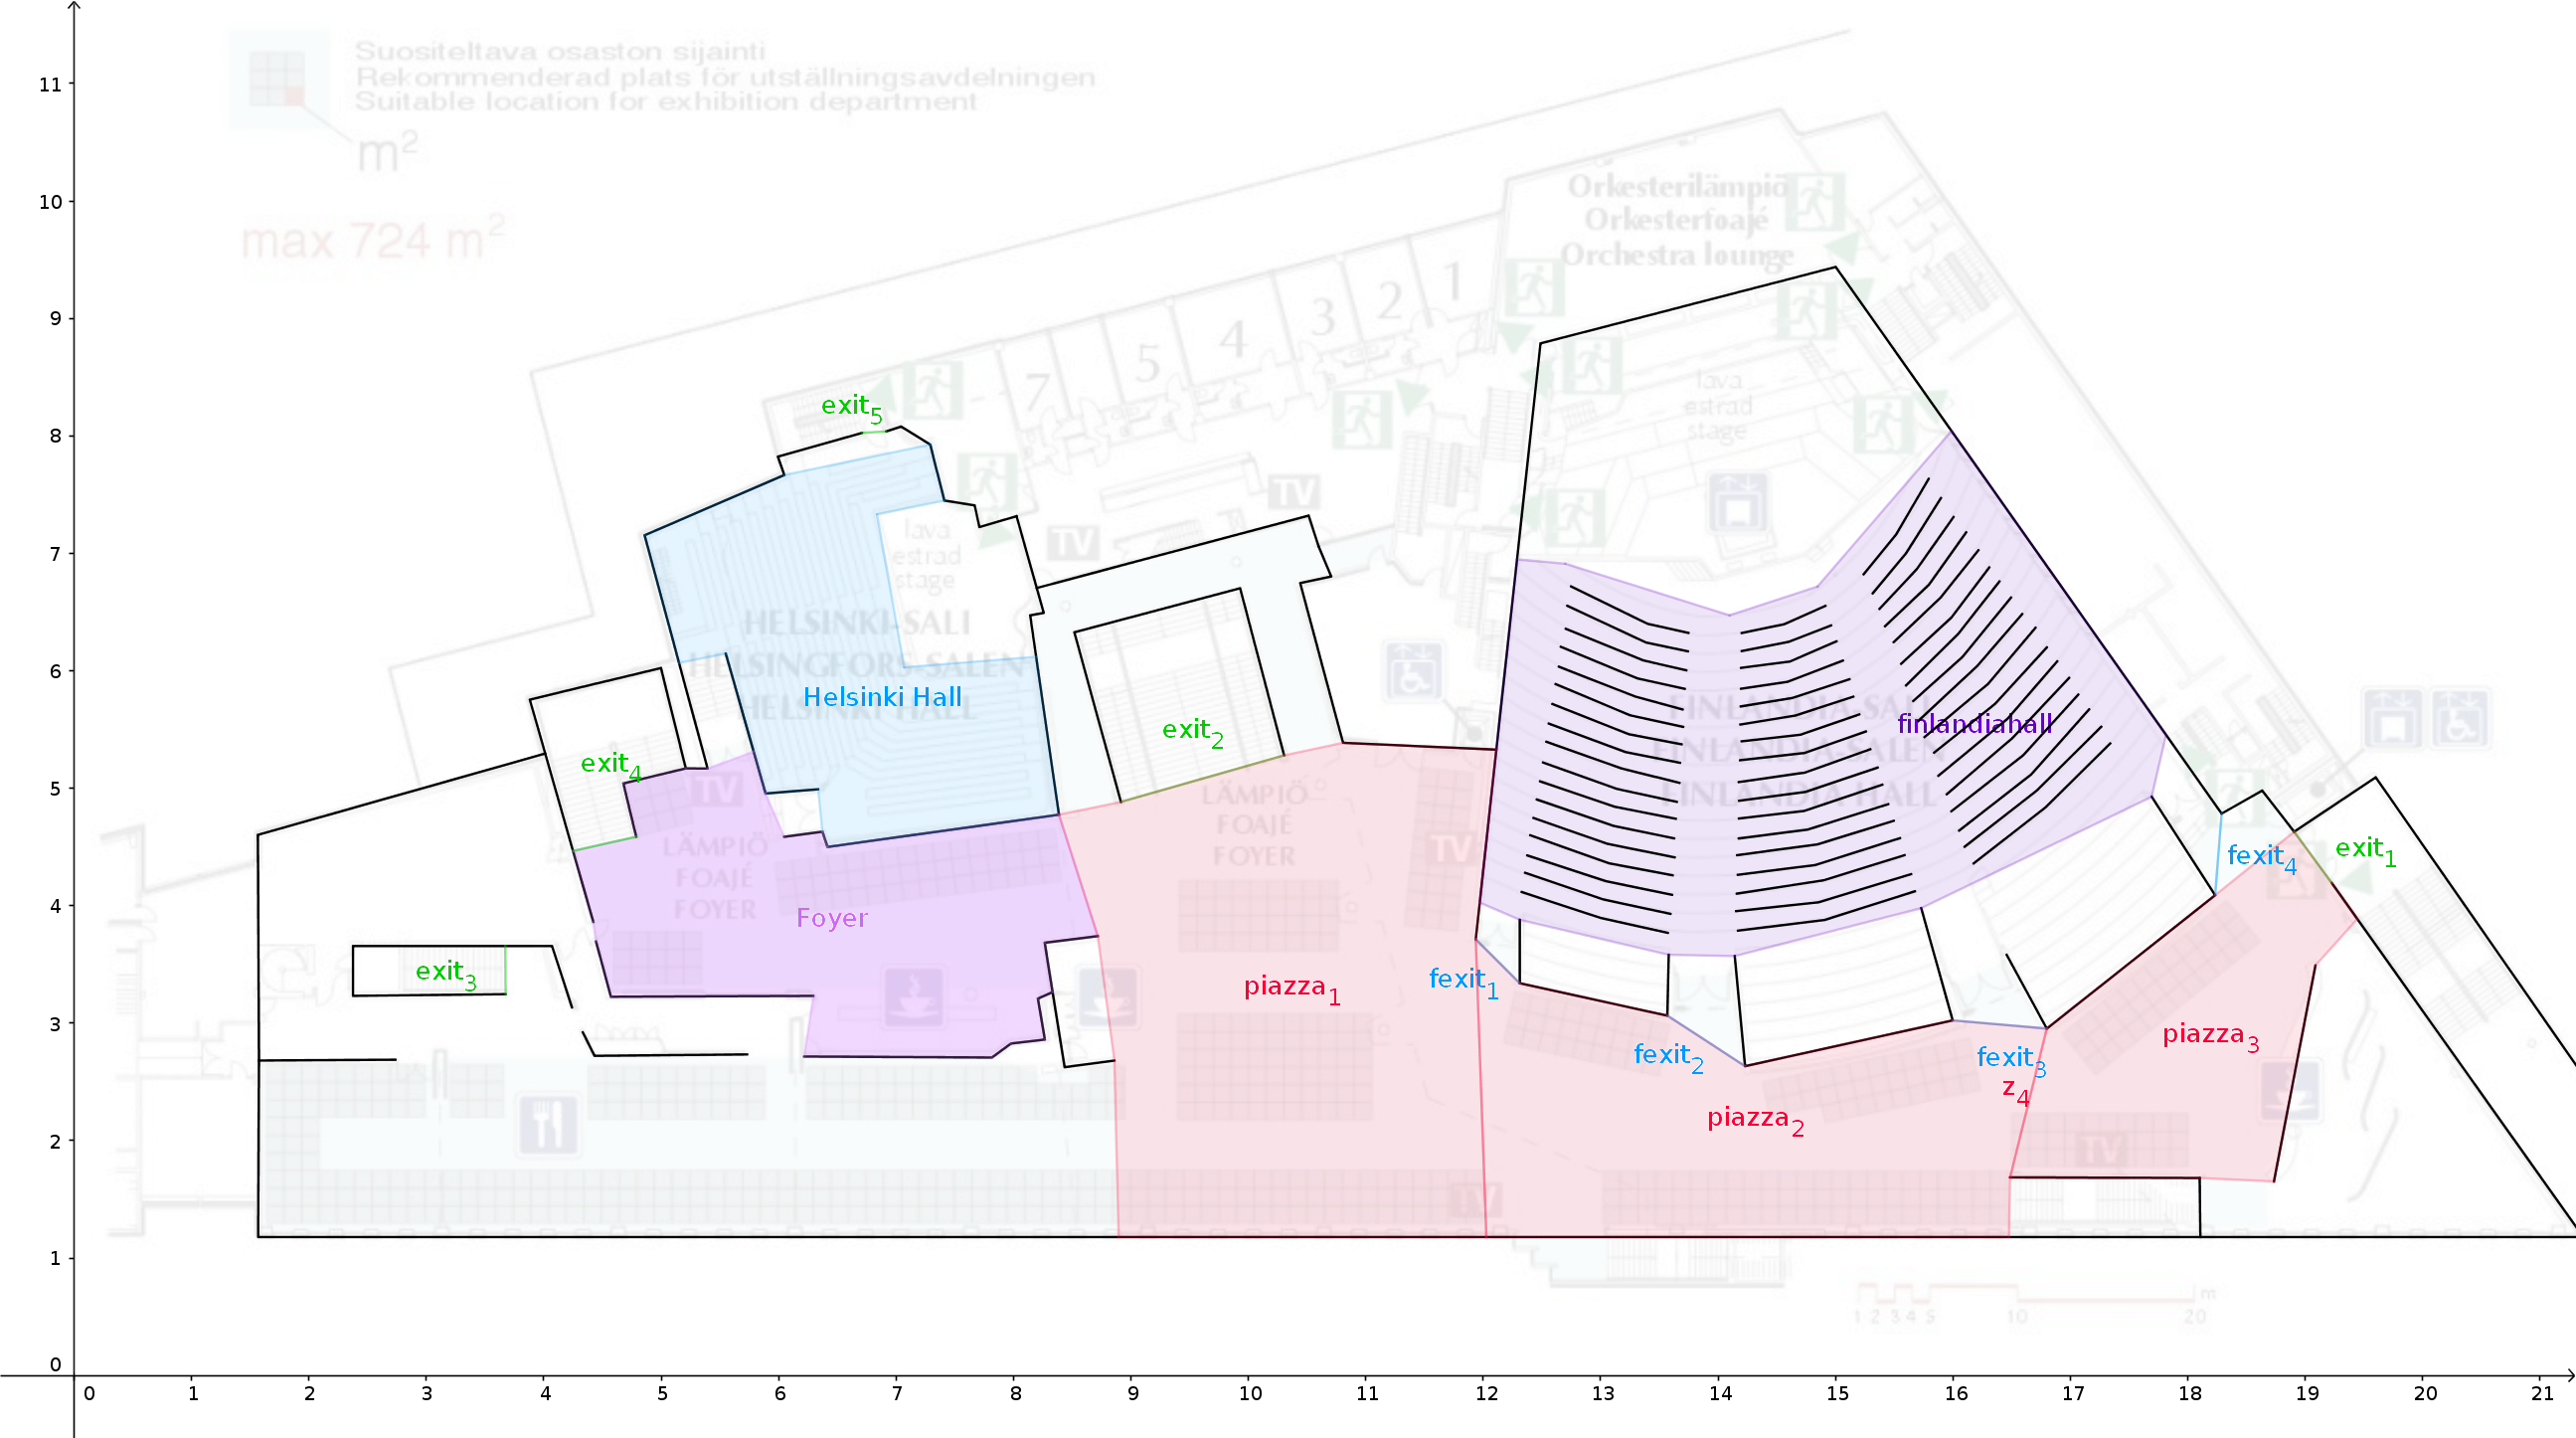
\includegraphics{./finlandia_talo.png}
\caption{\emph{Finlandia Talo}}
\end{figure}

\begin{center}\rule{0.5\linewidth}{\linethickness}\end{center}

\textbf{Description}

Genetic algorithm for optimizing the evacuation time of crowd of people
by placing leaders into the area \(S\).

\begin{center}\rule{0.5\linewidth}{\linethickness}\end{center}

\textbf{Initial values}

\begin{itemize}
\tightlist
\item
  \(k\) leaders.
\item
  \(m\) different non-empty disjoint regions from the area \(S\). We
  denote individual region by its index \(i ∈ \{1, ..., m\}\).
\item
  Population of size of \(n\) (simulations per generation).
\end{itemize}

Total number of combinations of placements of \(k\) leaders into \(m\)
regions.

\[ \binom{m}{k}, m ≥ k \]~

Each leader is also assigned a target that is one of the exits

\[ Targets = \{exit_i ∣ i ∈ \{1, 5\}\}\]

\begin{center}\rule{0.5\linewidth}{\linethickness}\end{center}

\textbf{Egress time distribution function}

\begin{itemize}
\tightlist
\item
  \(x\)-axis: Unit of time
\item
  \(y\)-axis: Number of agents that have reached the exit
\end{itemize}

\[ \frac{\text{number of agents that have reached the exit}}{\text{unit of time}} \]

\begin{center}\rule{0.5\linewidth}{\linethickness}\end{center}

\textbf{Genetic algorithm}

\begin{itemize}
\tightlist
\item
  \textbf{Individual}: Each suggested solution for a genetic algorithm.
  \emph{Each individual consists \(k\) number of \((region, target)\)
  tuples. Because leaders are indentical order does not matter.}
  \[ I = \{(region , target)_1,..., (region , target)_k\}\]
\item
  \textbf{Population}: The collection of unique individuals.
  \[ P = \{I_1, ...,I_n\}, I_i ≠ I_j \]
\item
  \textbf{Fitness function}: Measure of how effective each solution
  (individual) is. \emph{Some function that depends on the cumulative
  distribution of the egress times of agents. e.g minimize evacuation
  time of 95\% (to avoid pollution from outliers) of the agents.}
\item
  \textbf{Grade}: Population's average fitness.
\end{itemize}

Evolution of population. Advances one \textbf{generation} to the next
one closer to optimal solution defined by the fitness function. Each
cycle consists of

\begin{enumerate}
\def\labelenumi{\arabic{enumi})}
\item
  \textbf{Selection}: Take a portion of best performing individuals.
  Also randomly select lesser performing individuals for genetic
  diversity.
\item
  \textbf{Breeding}: Breed together parents to repopulate the population
  to its desired size.

  \emph{TODO ???}
\item
  \textbf{New population}: Merge together the parents and children to
  constitute the next generation's population.
\item
  \textbf{Random mutation}: Finally we mutate a small random portion of
  the population. What this means is to have a probability of randomly
  modifying each individual. \emph{Change the region where some leader
  is places of an random individual.}
\end{enumerate}

where the \textbf{parameters} are

\begin{itemize}
\tightlist
\item
  Percentage of best performing individual to retain into new
  generation. \[ p_{retain} \in [0, 1] \]
\item
  Change of random selection of lesser performing individual.
  \[ p_{selection} \in [0, 1] \]
\item
  Change of mutation. \[ p_{mutation} \in [0, 1] \]
\end{itemize}

\begin{center}\rule{0.5\linewidth}{\linethickness}\end{center}

\textbf{Implementation}

\begin{itemize}
\tightlist
\item
  Simulation exit condition depends on the chose fitness function
\item
  Memoize the values generated by simulation configurations
\end{itemize}
